%%
%% This is file `sigconf.tex',
%% generated with the docstrip utility.
%%
%% The original source files were:
%%
%% samples.dtx  (with options: `all,proceedings,sigconf')
%% 
%% IMPORTANT NOTICE:
%% 
%% For the copyright see the source file.
%% 
%% Any modified versions of this file must be renamed
%% with new filenames distinct from sigconf.tex.
%% 
%% For distribution of the original source see the terms
%% for copying and modification in the file samples.dtx.
%% 
%% This generated file may be distributed as long as the
%% original source files, as listed above, are part of the
%% same distribution. (The sources need not necessarily be
%% in the same archive or directory.)
%%
%%
%% Commands for TeXCount
%TC:macro \cite [option:text,text]
%TC:macro \citep [option:text,text]
%TC:macro \citet [option:text,text]
%TC:envir table 0 1
%TC:envir table* 0 1
%TC:envir tabular [ignore] word
%TC:envir displaymath 0 word
%TC:envir math 0 word
%TC:envir comment 0 0
%%
%% The first command in your LaTeX source must be the \documentclass
%% command.
%%
%% For submission and review of your manuscript please change the
%% command to \documentclass[manuscript, screen, review]{acmart}.
%%
%% When submitting camera ready or to TAPS, please change the command
%% to \documentclass[sigconf]{acmart} or whichever template is required
%% for your publication.
%%
%%
\documentclass[sigconf,anonymous,review]{acmart}
%% Table notes, so that each table states its own source and expands its own
%% acronyms without the reader having to find the surrounding text.
\usepackage{threeparttable}
%% Pseudocode for the fit of sec:structure_parameter_learning.  `\parState`
%% is a statement whose continuation lines keep the indentation of the block.
\usepackage{algorithm}
\usepackage{algpseudocode}
\makeatletter
\algnewcommand{\parState}[1]{\State%
  \parbox[t]{\dimexpr\linewidth-\ALG@thistlm}{\strut #1\strut}}
\makeatother
%%
%% \BibTeX command to typeset BibTeX logo in the docs
\AtBeginDocument{%
  \providecommand\BibTeX{{%
    Bib\TeX}}}

%% Rights management information.  This information is sent to you
%% when you complete the rights form.  These commands have SAMPLE
%% values in them; it is your responsibility as an author to replace
%% the commands and values with those provided to you when you
%% complete the rights form.
\setcopyright{acmlicensed}
\copyrightyear{2018}
\acmYear{2018}
\acmDOI{XXXXXXX.XXXXXXX}
%% These commands are for a PROCEEDINGS abstract or paper.
\acmConference[Conference acronym 'XX]{Make sure to enter the correct
  conference title from your rights confirmation email}{June 03--05,
  2018}{Woodstock, NY}
%%
%%  Uncomment \acmBooktitle if the title of the proceedings is different
%%  from ``Proceedings of ...''!
%%
%%\acmBooktitle{Woodstock '18: ACM Symposium on Neural Gaze Detection,
%%  June 03--05, 2018, Woodstock, NY}
\acmISBN{978-1-4503-XXXX-X/2018/06}


%%
%% Submission ID.
%% Use this when submitting an article to a sponsored event. You'll
%% receive a unique submission ID from the organizers
%% of the event, and this ID should be used as the parameter to this command.
%%\acmSubmissionID{123-A56-BU3}

%%
%% For managing citations, it is recommended to use bibliography
%% files in BibTeX format.
%%
%% You can then either use BibTeX with the ACM-Reference-Format style,
%% or BibLaTeX with the acmnumeric or acmauthoryear sytles, that include
%% support for advanced citation of software artefact from the
%% biblatex-software package, also separately available on CTAN.
%%
%% Look at the sample-*-biblatex.tex files for templates showcasing
%% the biblatex styles.
%%
%%
%% The majority of ACM publications use numbered citations and
%% references.  The command \citestyle{authoryear} switches to the
%% "author year" style.
%%
%% If you are preparing content for an event
%% sponsored by ACM SIGGRAPH, you must use the "author year" style of
%% citations and references.
%% Uncommenting
%% the next command will enable that style.
%%\citestyle{acmauthoryear}


%%
%% end of the preamble, start of the body of the document source.
\begin{document}

%%
%% The "title" command has an optional parameter,
%% allowing the author to define a "short title" to be used in page headers.
% \title{The Name of the Title Is Hope}
\title{N$^2$DBN: Nested Non-Stationary Dynamic Bayesian Networks}

%% Authors and affiliations are withheld for anonymous review.  The
%% `anonymous` class option typesets the anonymous byline, and the real
%% metadata is restored in the camera-ready version.

%%
%% The abstract is a short summary of the work to be presented in the
%% article.
\begin{abstract}
Web, mobile, and wearable systems log human activity as timestamped events with durations. Dynamic Bayesian network (DBN) structure learning identifies such dependencies, and standard formulations fix one granularity and assume stationarity. Human activity logs violate both, since dependence changes over time and behaviors span minutes to weeks, and fitting one granularity at a time gives disagreeing answers. We present the nested non-stationary dynamic Bayesian network (N$^2$DBN) which models event starts and durations jointly under a zero-inflated negative binomial emission at the coarsest resolution and constrained Dirichlet-multinomial allocation below it, so coarser counts are deterministic sums needing no reconciliation. A regime chain and a latent factor model the non-stationarity, and variational Structural Expectation-Maximization with resolution-aware search learns the graph top-down across scales. In simulated experiments with ground truth, it recovers more structure than eight published learners, among them hill climbing, exhaustive search, greedy equivalence search, and Peter-Clark. It alone reaches a structural error below the empty graph's, and on a declared-pattern benchmark matches them with far fewer spurious edges. Applied to LifeSnaps, it places every calendar relation on the hour scale and every persistence relation on the day and week scales, and its simulated logs match observed counts and durations four times closer than an intercept baseline, preserving trend, drift and week scale changepoints (F\_1 = 0.96). In the QuitoBench application traffic forecasting benchmark, accuracy was close to the state of the art, behind the PatchTST transformer by $23\%$ and DLinear by 26\%, while its cross-scale coherence is much better, $8\times10^{-15}\%$ against their 4 to 5\%. We demonstrate that N²DBN learns structure from human behavior event logs, simulates faithful replicas, and forecasts them coherently.
\end{abstract}

%%
%% The code below is generated by the tool at http://dl.acm.org/ccs.cfm.
%% Please copy and paste the code instead of the example below.
%%
\begin{CCSXML}
<ccs2012>
   <concept>
       <concept_id>10002950.10003648.10003649.10003650</concept_id>
       <concept_desc>Mathematics of computing~Bayesian networks</concept_desc>
       <concept_significance>500</concept_significance>
       </concept>
   <concept>
       <concept_id>10002950.10003648.10003688.10003693</concept_id>
       <concept_desc>Mathematics of computing~Time series analysis</concept_desc>
       <concept_significance>500</concept_significance>
       </concept>
   <concept>
       <concept_id>10010147.10010341.10010349.10010361</concept_id>
       <concept_desc>Computing methodologies~Multiscale systems</concept_desc>
       <concept_significance>500</concept_significance>
       </concept>
   <concept>
       <concept_id>10003120.10003138</concept_id>
       <concept_desc>Human-centered computing~Ubiquitous and mobile computing</concept_desc>
       <concept_significance>500</concept_significance>
       </concept>
   <concept>
       <concept_id>10010147.10010257</concept_id>
       <concept_desc>Computing methodologies~Machine learning</concept_desc>
       <concept_significance>300</concept_significance>
       </concept>
 </ccs2012>
\end{CCSXML}

\ccsdesc[500]{Mathematics of computing~Bayesian networks}
\ccsdesc[500]{Mathematics of computing~Time series analysis}
\ccsdesc[500]{Computing methodologies~Multiscale systems}
\ccsdesc[500]{Human-centered computing~Ubiquitous and mobile computing}
\ccsdesc[300]{Computing methodologies~Machine learning}
% \ccsdesc[500]{Do Not Use This Code~Generate the Correct Terms for Your Paper}
% \ccsdesc[300]{Do Not Use This Code~Generate the Correct Terms for Your Paper}
% \ccsdesc{Do Not Use This Code~Generate the Correct Terms for Your Paper}
% \ccsdesc[100]{Do Not Use This Code~Generate the Correct Terms for Your Paper}

%%
%% Keywords. The author(s) should pick words that accurately describe
%% the work being presented. Separate the keywords with commas.
\keywords{dynamic Bayesian networks, non-stationary time series, multiscale modeling, human behavior modeling}
\received{24 August 2026}
% \received[revised]{}
% \received[accepted]{}

%%
%% This command processes the author and affiliation and title
%% information and builds the first part of the formatted document.
\maketitle



\section{Introduction}
\label{sec:introduction}
A behavioral event log records the start times and durations of labeled activity episodes, such as user interactions with mobile applications, website visits, or periods of physical activity captured by wearable sensors. The structure that emerges from such a log depends on the temporal lens through which we examine it. At the scale of minutes, we observe individual episode onsets. At the scale of hours, the same data are more naturally characterized by episode counts and the total time spent in each activity. At the scale of days or weeks, the log reveals broader behavioral patterns, such as non-stationary behavior including trends and seasonal effects, while abstracting away most fine-grained temporal detail. Therefore, by examining the same event log from different temporal perspectives, we can observe distinct patterns at different timescales. Each coarser temporal view must be an aggregation of a finer one, resulting in a nested hierarchy of mutually consistent temporal scales.

\begin{figure}[h]
  \centering
  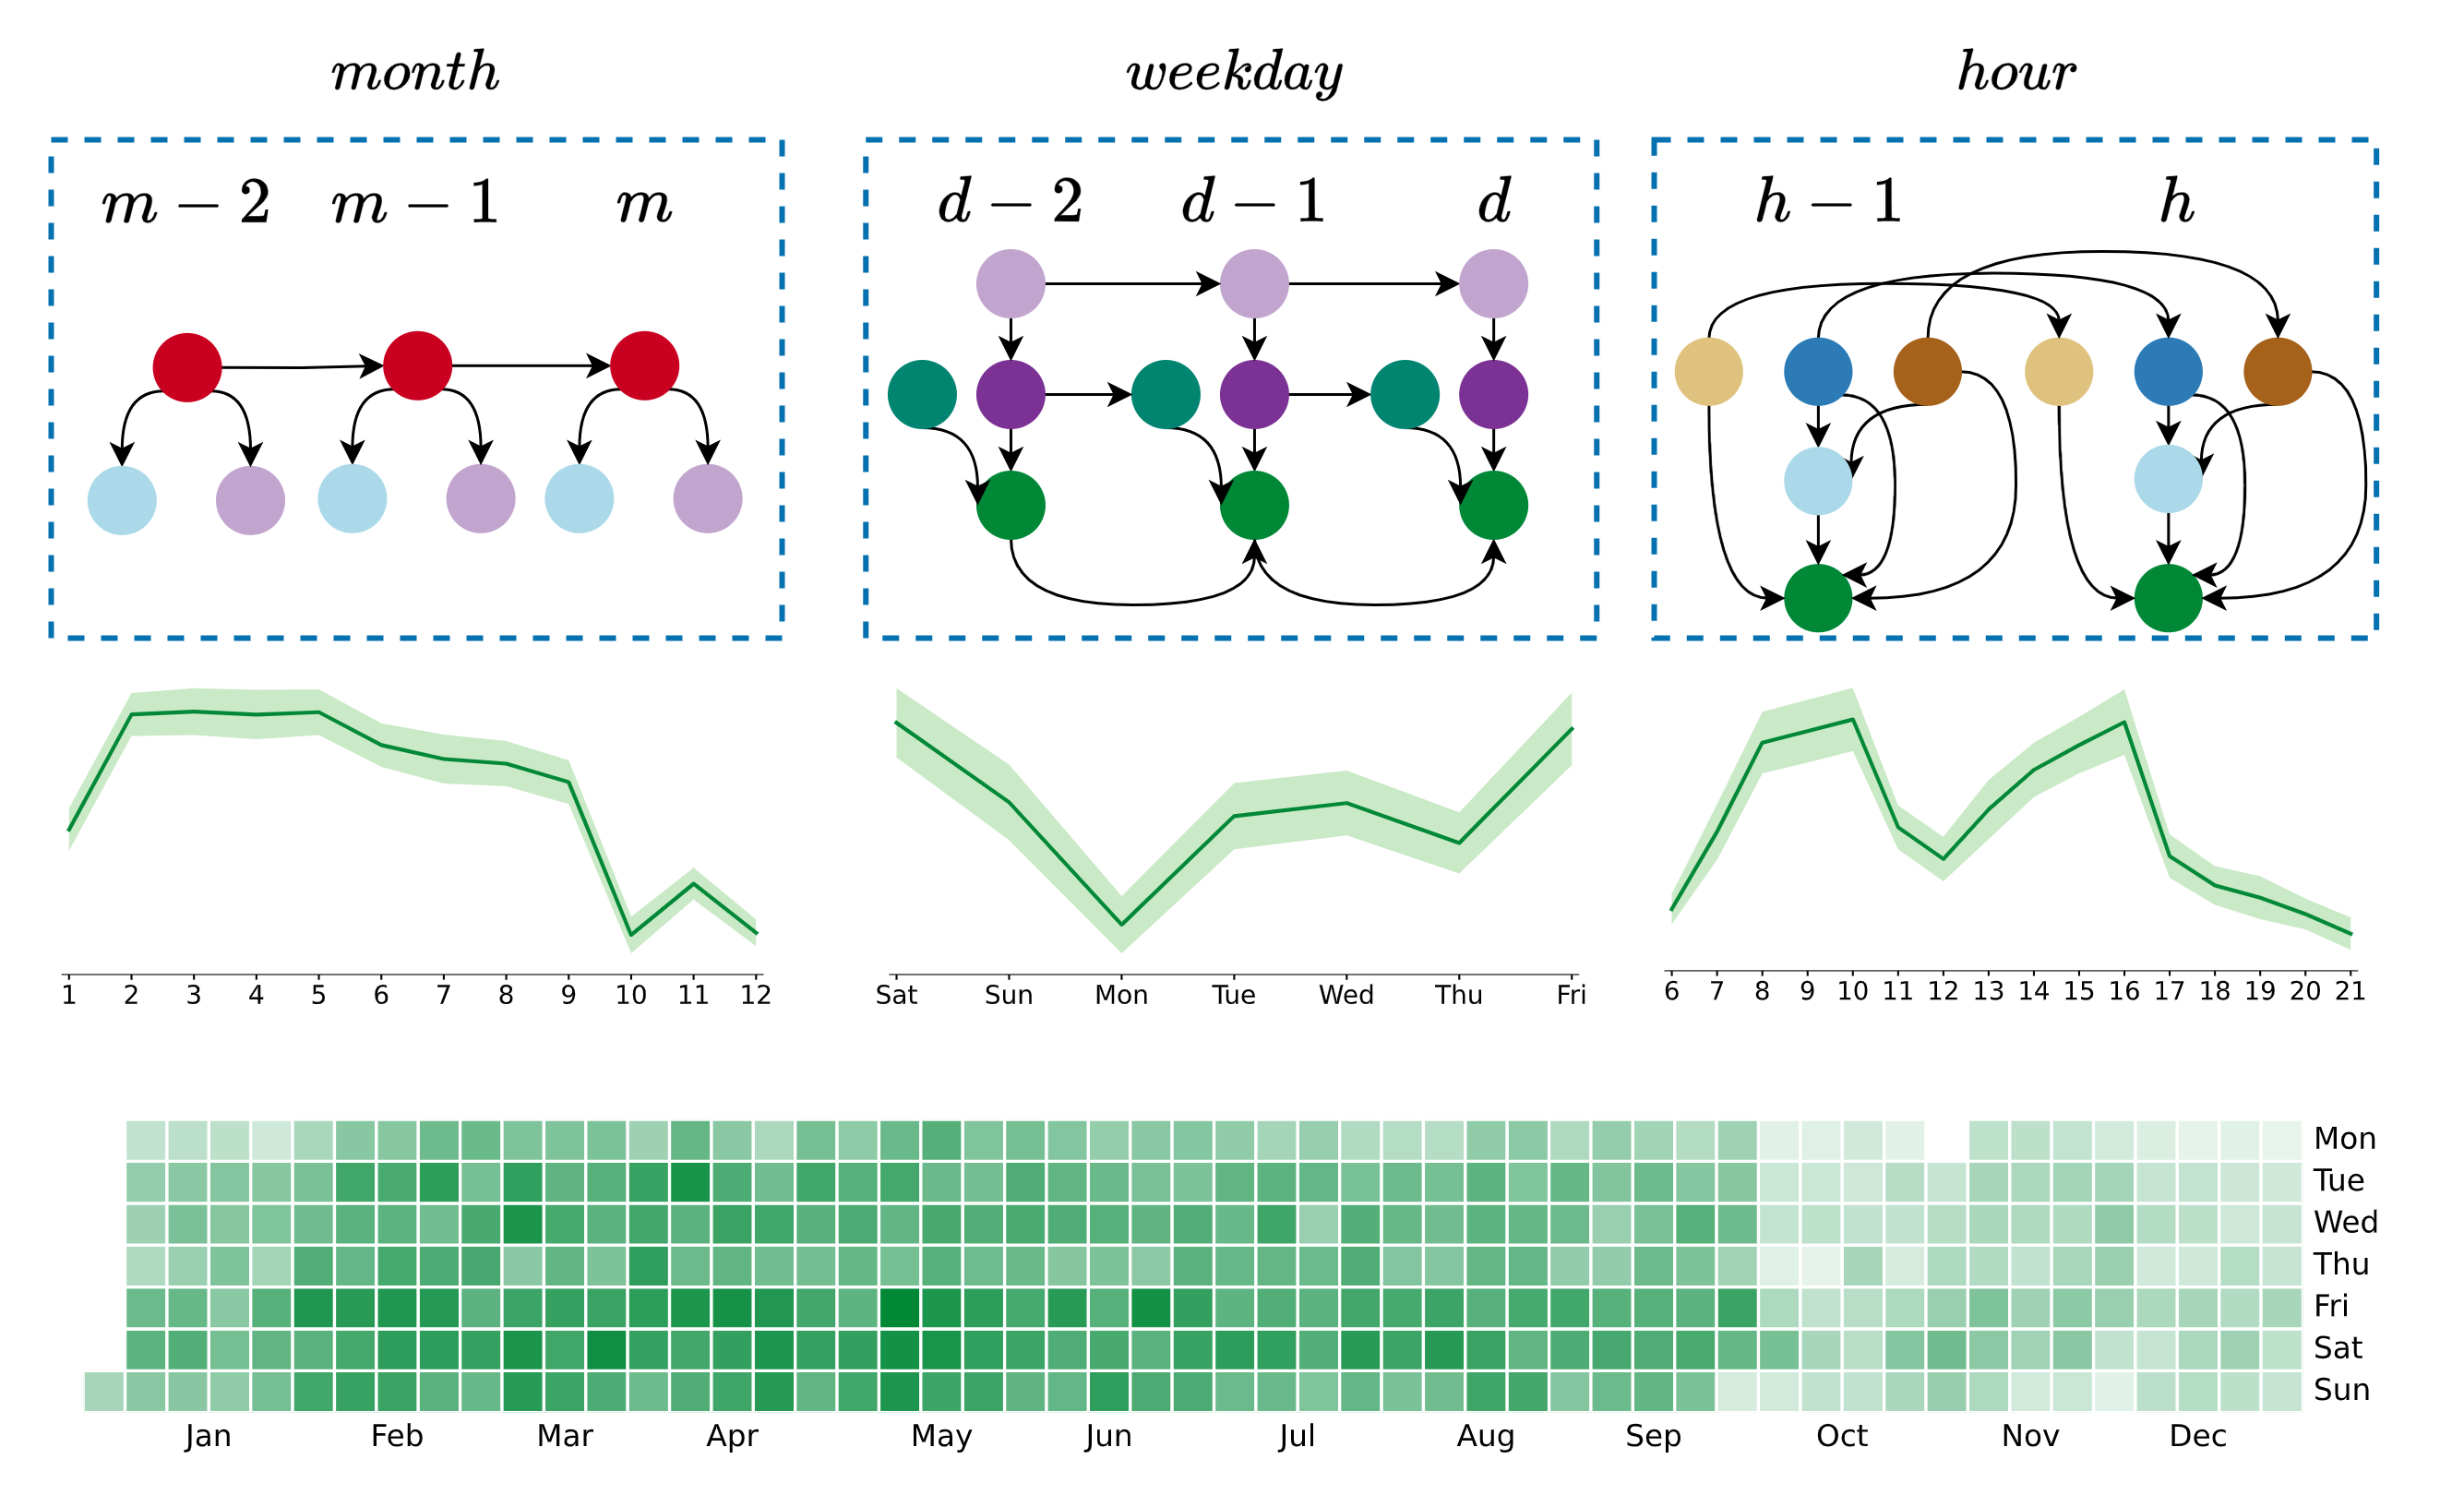
\includegraphics[width=\columnwidth]{n2dbn.png}
\caption{Progression of human behavior across timescales, the focus of non-stationary dynamic Bayesian networks (N$^2$DBN).}
  % \Description{Enjoying the baseball game from the third-base
  % seats. Ichiro Suzuki preparing to bat.}
  \label{fig:teaser}
\end{figure}

Dynamic Bayesian networks (DBNs) are the natural starting point. DBNs are directed probabilistic graphical models for temporal stochastic processes. They represent the joint distribution over time in a factored form, can include observed and latent variables, and make temporal dependencies interpretable through their graph structure \citep{murphy_2002_dbn}. DBN structure learning extends Bayesian network structure learning to time-lagged trajectories, using the same broad score-based, constraint-based and hybrid optimization-based families \citep{kitson_survey_2023,kungurtsev_learning_2025}. However, standard DBNs are specified at a chosen time granularity; changing the granularity changes the transition model, so DBNs fitted separately at hourly and daily resolutions are not automatically constrained to agree under aggregation or marginalization \citep{saria_reasoning_2007}. This leaves a central modeling gap. A framework for event logs must represent non-stationary dependencies at their relevant timescales while preserving exact aggregation relationships across temporal resolutions.

N$^2$DBN addresses this gap within a single generative formulation. It defines the likelihood once at the configured finest temporal resolution over event starts and their durations, and represents counts and durations at every coarser resolution as deterministic aggregations of these quantities. Non-stationary components and temporal dependencies can therefore be evaluated at their respective timescales without fitting independent models that may disagree on their implied aggregates. A resolution-aware variational Structural Expectation-Maximization (SEM) procedure jointly learns the dependency structure under these constraints. Thus, N$^2$DBN incorporates cross-resolution consistency into the probabilistic model itself, so separately estimated temporal views never have to be reconciled.

The remainder of this paper is organized as follows. Section~\ref{sec:related-work} reviews related work. Section~\ref{sec:preliminaries} formulates the problem and introduces N$^2$DBN. Section~\ref{sec:methodology} presents the proposed structure- and parameter-learning algorithm. Section~\ref{sec:experiments} evaluates the modeling fidelity and structure-learning accuracy of N$^2$DBN through extensive experiments. Section~\ref{sec:case-study} presents a case study on the LifeSnaps dataset, an observed log with no ground-truth graph, and grades the learned structure, the fidelity of the simulated log and the preservation of its non-stationary patterns. Finally, Section~\ref{sec:conclusions} concludes the paper.

\section{Related Work}
\label{sec:related-work}

Researchers have extended Bayesian network learning to temporal processes by identifying dependencies within and across consecutive time slices to enable DBN structure learning. Classical approaches include score-based search, constraint-based methods, and hybrid procedures, while SEM provides a framework for structure learning in the presence of missing or latent variables \citep{murphy_2002_dbn,kitson_survey_2023,kungurtsev_learning_2025}. In the standard discrete-time formulation, the temporal model is defined relative to a selected time epoch and the learned transition structure is applied at that resolution. Consequently, changing the discretization changes the variables, sufficient statistics, and potentially the learned dependency structure.
% Although these methods provide general mechanisms for identifying temporal dependencies, they do not explicitly couple structure learning across nested temporal resolutions.

Some researchers have relaxed the stationarity assumption of conventional DBNs. Non-stationary DBNs based on change-point processes divide a trajectory into segments and allow model parameters, and in some cases network structures, to vary between segments \citep{grzegorczyk_nonstationary_2009}. Time-varying DBNs instead allow the directed dependency structure to evolve more continuously, for example through kernel-reweighted sparse autoregressive estimation under an assumption of smooth structural variation \citep{song_timevarying_2009}. Subsequent non-homogeneous DBN formulations further share information between adjacent segments by coupling interaction parameters, including edge-wise schemes that determine which dependencies remain stable and which change over time \citep{kamalabad_nonhomogeneous_2020}. These approaches address an important limitation of homogeneous DBNs by representing temporal variation in parameters or structure. However, the variation is modeled along a single temporal representation of the data.
% They do not jointly constrain models defined at finer and coarser temporal resolutions to represent aggregations of the same underlying process.

Multi-scale temporal modeling has been studied from several complementary perspectives. In temporal graphical models, \citet{saria_reasoning_2007} noted that conventional DBNs operate at a fixed time granularity and developed an inference procedure for continuous-time Bayesian networks in which different clusters can be approximated at different temporal resolutions. This approach adapts the granularity of inference to the rates at which different components evolve. It constructs no hierarchy of aggregated observations. Kang et al.~\citep{kang_multiscale_2022} took a different approach, combining dynamic network inference with recursive temporal partitioning. Their framework detects changes in conditional dependencies at multiple temporal scales by partitioning a non-stationary series into locally stationary intervals and fitting sparse vector autoregressive (VAR) networks within those intervals.

Moreover, researchers have explored multi-scale modeling outside the field of DBN structure learning. ProbRules, for example, integrates biological mechanisms operating at different rates through probabilistic rules \citep{gross_multiscale_2019}, while recent neural architectures such as DynaMamba construct pyramidal representations by progressively down-sampling a time series and fusing information across resolutions \citep{chen_dynamamba_2026}. These methods demonstrate the value of representing temporal phenomena at more than one scale.
% but their notions of scale concern adaptive inference, temporal partitioning, mechanism-specific rates, or learned feature representations. They do not impose an aggregation identity under which quantities at every coarser temporal resolution are deterministic functions of a common finest-scale stochastic process.

The requirement that predictions remain consistent across a hierarchy has been studied explicitly in hierarchical time-series forecasting. In this setting, series are organized in a predefined hierarchy in which values at parent nodes equal sums of their children. Traditional approaches first produce forecasts independently and subsequently reconcile them to satisfy these aggregation constraints, whereas end-to-end and top-down probabilistic models can enforce coherence by construction \citep{das_topdown_2023}. This concept is closely related to the consistency requirement considered in our work, but the hierarchy has a different meaning. Hierarchical forecasting primarily relates distinct series through a cross-sectional aggregation structure at a common temporal index. Our setting instead concerns \emph{temporal aggregation of the same event process}; for example, hourly activity counts and durations must equal the corresponding sums of their constituent fine-resolution intervals. Moreover, hierarchical forecasting addresses prediction under a known aggregation hierarchy. Learning directed temporal dependencies among event processes lies outside its scope.

Taken together, these lines of research address complementary aspects of the problem: DBN methods learn temporal dependency structure, non-stationary DBNs allow dependencies or their strengths to evolve over time, multi-scale models capture phenomena at different temporal resolutions, and hierarchical forecasting provides mechanisms for aggregation coherence. However, they do not jointly learn directed, non-stationary dependencies across nested temporal resolutions while deriving every coarser observation from the same fine-resolution event process. N$^2$DBN is designed to fill this gap.

\section{Preliminaries}
\label{sec:preliminaries}

Here, we introduce the notation and constraints used to formulate the problem of learning behavioral dynamics across nested temporal resolutions.

\subsection{Problem Formulation}
\label{sec:problem_formulation}

Let temporal resolutions (e.g., hour, day, week) be indexed by \(k \in \{1,\dots,K\}\), with \(k=1\) the finest resolution and \(k=K\) the coarsest. For each timescale \(k\), we define \(t\in\mathcal{T}^{(k)} = \{1,\dots,T_k\}\) as the ordered set of epochs at scale \(k\) over the study horizon, where \(T_k \in \mathbb{N}\) is the number of such epochs. For each \(k \in \{1,\dots,K-1\}\), a surjective parent map \(\pi_k : \mathcal{T}^{(k)} \to \mathcal{T}^{(k+1)}\) sends each epoch at scale \(k\) to the unique epoch at scale \(k+1\) that contains it. For \(c \in \mathcal{T}^{(k+1)}\), its set of child epochs is \(\operatorname{ch}_k(c) = \{\,t \in \mathcal{T}^{(k)} : \pi_k(t) = c\,\}\).

An epoch at scale \(k\) is a contiguous interval of wall-clock time, and the child sets partition the epochs of scale \(k\) into blocks, one block per parent epoch. Let \(n_k\) denote the number of finest-scale epochs contained in one epoch at scale \(k\). Thus, \(n_1=1\) and, when the hierarchy is regular, \(n_{k+1} = n_k\lvert\operatorname{ch}_k(c)\rvert\). A finest-scale epoch is called a \emph{slot}. Durations at every scale are counted in slots, so one unit of duration has the wall-clock length of one slot. For \(k<j\), composing the parent maps gives \(\pi_{j-1} \circ \cdots \circ \pi_k\), which associates each scale-\(k\) epoch with the scale-\(j\) epoch containing it. Each scale-\(j\) epoch therefore comprises the scale-\(k\) epochs nested within it. The hierarchy is a fixed, known input that encodes the calendar, such as slots, hours, days, and weeks; ergo not estimated.

Let \(\mathcal{L}\) be the finite set of event labels, with \(L=\lvert\mathcal{L}\rvert\). For each scale \(k\), epoch \(t \in \mathcal{T}^{(k)}\), and label \(\ell \in \mathcal{L}\), the observed variable \(X_t^{(k,\ell)} \in \mathbb{N}_0\) records the number of episodes of label \(\ell\) that start in epoch \(t\), while \(Y_t^{(k,\ell)} \in \mathbb{N}_0\) records the total duration, measured in slots, of those episodes. Each epoch also has a vector of observed context features \(\mathcal{K}_t^{(k)} \in \mathbb{R}^{d_k}\), such as calendar position, season, or intervention status.

Counting durations in slots keeps both observed channels on the integer lattice, allowing the same allocation law to be used for counts and durations at every scale. The full duration of an episode is assigned to the epoch in which that episode starts. Therefore, \(Y_t^{(k,\ell)}\) may include a duration that extends beyond the end of epoch \(t\); it does not represent only the time for which label \(\ell\) is active within that epoch. Two structural constraints follow from this finest-scale representation.

First, the atomic start and duration support is
\begin{equation}
  \begin{aligned}
    X_t^{(1,\ell)}&\in\{0,1\}, &
    0\leq X_t^{(k,\ell)}&\leq n_k,\\
    X_t^{(k,\ell)}=0&\Longleftrightarrow
    Y_t^{(k,\ell)}=0, &
    Y_t^{(k,\ell)}&\geq X_t^{(k,\ell)}.
  \end{aligned}
  \label{eq:atomic_support}
\end{equation}
so the slot width permits at most one start per label, an epoch without a start has no booked duration, and every start contributes at least one slot of duration. Second, counts and durations agree under every adjacent aggregation,
\begin{align}
  X_c^{(k+1,\ell)}
  &=\sum_{t\in\operatorname{ch}_k(c)}X_t^{(k,\ell)}, &
  Y_c^{(k+1,\ell)}
  &=\sum_{t\in\operatorname{ch}_k(c)}Y_t^{(k,\ell)}.
  \label{eq:aggregation_constraints}
\end{align}
Having \(\mathcal{A}\) as the deterministic aggregation operator and \(Z^{(k)}=(X^{(k)},Y^{(k)})\) the whole fine-scale array, the known fold will be \((\mathcal{A}_kZ^{(k)})_c=\sum_{t\in\operatorname{ch}_k(c)}Z_t^{(k)}\). Its admissible fiber is
\begin{equation*}
  \mathcal F_k(v)=\{u:\mathcal A_ku=v\text{ and }u
  \text{ satisfies Equation~\eqref{eq:atomic_support}}\}.
\end{equation*}
Thus, \(Z^{(k+1)}=\mathcal{A}_kZ^{(k)}\), and \(\mathcal F_k(v)\) contains exactly the admissible fine allocations of \(v\).

Given \(Z^{(1:K)}\), \(\mathcal K^{(1:K)}\), and the fixed hierarchy, the problem is to estimate a resolution-specific temporal graph \(\mathcal G=\{\mathcal G^{(k)}\}_{k=1}^{K}\) and conditional parameters \(\Theta=\{\Theta^{(k)}\}_{k=1}^{K}\). The model must explain starts and durations jointly, distinguish lagged dependence from persistent change and same-epoch co-movement, and assign probability only to arrays that satisfy the aggregation identities. Let \(\mathfrak G_{\mathrm{adm}}\) be the set of positive-lag graphs defined by the declared maximum lags and in-degree bounds, and let \(\mathcal E^{(k)}\) be the learned edges at scale \(k\). The estimation problem is
\begin{align}
  (\widehat\Theta,\widehat{\mathcal G})
  =\arg\max_{\substack{\Theta\\
  \mathcal G\in\mathfrak G_{\mathrm{adm}}}}
  \Big[&\log p_{\Theta,\mathcal G}
  (Z^{(1:K)}\mid\mathcal K^{(1:K)})\nonumber\\[-2pt]
  &-\sum_{k=1}^{K}\lambda_k|\mathcal E^{(k)}|\Big],
  \label{eq:problem_objective}
\end{align}
where \(\lambda_k\) is the penalty on an edge at scale \(k\). In addition, every distribution allowed by Equation~\eqref{eq:problem_objective} must satisfy \(\mathcal A_{j-1}\cdots\mathcal A_kZ^{(k)}=Z^{(j)}\) almost surely for every \(k<j\). The required output is therefore one learned multiresolution model in which the graph, parameters, latent progression, forecasts, and generated event logs remain consistent with the same observed event process.

\section{Methodology}
\label{sec:methodology}

This section presents N$^2$DBN as the model used to solve Equation~\eqref{eq:problem_objective}. We first define its nested generative construction, latent states, and resolution-specific temporal graphs. We then describe the variational Structural Expectation-Maximization (vSEM) procedure for inferring the latent trajectories and learning the conditional parameters and graph structure.

\subsection{Nested Generative Model}
\label{sec:nested_generative_model}

At scale \(k\), let \(p_k\in\mathbb N\) be the maximum admissible lag. For a target label \(\ell\in\mathcal L\), let \(\mathcal C_{k,\ell}\subseteq\mathcal L\times\{1,\ldots,p_k\}\) be its set of candidate parents. A candidate \((a,d)\) identifies source label \(a\) and a positive lag of \(d\) scale-\(k\) epochs, so its count and duration values at target epoch \(t\) are \(X_{t-d}^{(k,a)}\) and \(Y_{t-d}^{(k,a)}\). N$^2$DBN learns the parent set \(\mathcal P_{k,\ell}\subseteq\mathcal C_{k,\ell}\) subject to \(|\mathcal P_{k,\ell}|\leq D_k\), where \(D_k\) is the maximum in-degree.

For scale \(k\), epoch \(t\), and target label \(\ell\), let \(\eta_{t,\ell}^{(k)}\in\mathbb R\) be the count predictor score and let \(\zeta_{t,\ell}^{(k)}\in\mathbb R\) be the duration predictor score. Each selected parent \((a,d)\in\mathcal P_{k,\ell}\) contributes separately to these two scores,
\begin{align}
  \eta_{t,\ell}^{(k)}
  &=\cdots+\beta_{a,d}^{(k,\ell)}
  \log(1+X_{t-d}^{(k,a)}),
  \nonumber\\
  \zeta_{t,\ell}^{(k)}
  &=\cdots+\alpha_{a,d}^{(k,\ell)}
  \log(1+Y_{t-d}^{(k,a)}).
  \label{eq:lagged_parent_terms}
\end{align}
The ellipses in Equation~\eqref{eq:lagged_parent_terms} contain the remaining additive terms, including the intercept, context, latent-state effects, and contributions from other selected parents. Thus, \(\eta_{t,\ell}^{(k)}\) and \(\zeta_{t,\ell}^{(k)}\) are real-valued intermediate scores. A predicted count or duration is obtained from them by the transformations that follow. At the coarsest scale, exponentiation converts them into the negative-binomial count-component and duration-surplus means. At finer scales, block softmax functions convert them into allocation weights. The \(\log(1+\cdot)\) transformation allows zero values and moderates the influence of large counts and durations. The coefficients \(\beta_{a,d}^{(k,\ell)}\) and \(\alpha_{a,d}^{(k,\ell)}\) are fitted from all scale-\(k\) epochs during the structure-learning step described in Section~\ref{sec:structure_parameter_learning}.

At the coarsest scale \(k=K\), let \(\varpi_t^{(K,\ell)}\in[0,1]\) be the structural-zero probability, let \(\phi_\ell^{(K)}>0\) be the count dispersion, and let \(\mu_t^{(K,\ell)}=\exp(\eta_{t,\ell}^{(K)})\) be the mean of the negative-binomial count component. The count emission draws an uncapped value and applies the count capacity,
\begin{equation}
  \begin{aligned}
    \widetilde X_t^{(K,\ell)}&\sim\operatorname{ZINB}
    \bigl(\varpi_t^{(K,\ell)},\phi_\ell^{(K)},
    \mu_t^{(K,\ell)}\bigr),\\
    X_t^{(K,\ell)}&=\min\{\widetilde X_t^{(K,\ell)},n_K\}.
  \end{aligned}
  \label{eq:coarsest_zinb}
\end{equation}
The zero-inflated negative binomial (ZINB) distribution is a mixture. With probability \(\varpi_t^{(K,\ell)}\), it generates a structural zero. With probability \(1-\varpi_t^{(K,\ell)}\), it draws from the negative-binomial component, which may also generate zero. Consequently, \(P(X=0)=\varpi+(1-\varpi)P_{\mathrm{NB}}(0)\). The cap ensures \(0\leq X_t^{(K,\ell)}\leq n_K\). The log-odds \(\log\{\varpi/(1-\varpi)\}\) is fitted from intercept, context, and latent-state effects and contains no selected lagged-parent term. A learned lag therefore affects the coarsest count distribution through \(\mu\).

For the duration channel, let \(s_\ell^{(K)}>0\) be the duration dispersion and let \(\nu_t^{(K,\ell)}=\exp(\zeta_{t,\ell}^{(K)})\) be the mean duration surplus. Conditional on \(X_t^{(K,\ell)}>0\), draw \(R_t^{(K,\ell)}\sim\operatorname{NB}(s_\ell^{(K)},\nu_t^{(K,\ell)})\) and define
\begin{equation}
  Y_t^{(K,\ell)}=
  \begin{cases}
    0, & X_t^{(K,\ell)}=0,\\
    X_t^{(K,\ell)}+R_t^{(K,\ell)},
      & X_t^{(K,\ell)}>0.
  \end{cases}
  \label{eq:coarsest_duration}
\end{equation}
This construction places the coarsest emission inside the support of Equation~\eqref{eq:atomic_support}.

Consider a two-scale hierarchy in which \(k=1\) denotes days and \(k=2\) denotes weeks. Let \(\mathrm{notification}\) be the source label, \(\mathrm{walk}\) the target label, and let the lag be one. At the weekly scale, this lag refers to the preceding week. Suppose that the other count terms sum to \(-0.3\), the notification-to-walk count coefficient is \(\beta_{\mathrm{notification},1}^{(2,\mathrm{walk})}=0.8\), and the preceding week contains \(X_{t-1}^{(2,\mathrm{notification})}=2\) notifications. The weekly walk-count score is then
\begin{equation*}
  \eta_{t,\mathrm{walk}}^{(2)}
  =-0.3+0.8\log(1+2)\approx0.579.
\end{equation*}
The negative-binomial count component has mean \(\exp(0.579)\approx1.78\) weekly walk episodes. The structural-zero probability \(\varpi_t^{(2,\mathrm{walk})}\) is determined by its separate predictor. With no notification in the preceding week, the count-component mean is \(\exp(-0.3)\approx0.74\). For duration, suppose that the other terms sum to \(1.0\), the notification-to-walk duration coefficient is \(\alpha_{\mathrm{notification},1}^{(2,\mathrm{walk})}=0.4\), and the preceding-week notification duration is \(Y_{t-1}^{(2,\mathrm{notification})}=5\) slots. This gives
\begin{equation*}
  \zeta_{t,\mathrm{walk}}^{(2)}
  =1.0+0.4\log(1+5)\approx1.717,
\end{equation*}
and a conditional mean duration surplus of \(\exp(1.717)\approx5.57\) slots. For a generated weekly walk count \(X_t^{(2,\mathrm{walk})}>0\), the corresponding conditional total-duration mean is \(X_t^{(2,\mathrm{walk})}+5.57\) slots.

At the daily scale \(k=1\), lag one refers to the preceding day, and the scores allocate a generated weekly total among its seven days. Suppose that Wednesday has walk-count score \(\eta_{\mathrm{Wed},\mathrm{walk}}^{(1)}=0.6\) after Tuesday's notification contribution is included, while each of the other six days has score zero. Wednesday's softmax weight is \(\exp(0.6)/(\exp(0.6)+6)\approx0.233\), and each other day has weight \(1/(\exp(0.6)+6)\approx0.128\). For a weekly total of four walk episodes, the unconstrained Dirichlet--multinomial reference means are \(4(0.233)\approx0.93\) episodes for Wednesday and \(4(0.128)\approx0.51\) for each other day. The kernel \(W_1\) uses these weights but generates only feasible integer allocations in \(\mathcal F_1\). Every draw sums to four, each daily count is at most \(n_1=1\), and the count and duration pair satisfies Equation~\eqref{eq:atomic_support}. Its constrained conditional means therefore need not equal the reference values. Hence, for the walk target, lag one means one week at scale 2 and one day at scale 1. The collection \(\mathcal G=\{\mathcal P_{k,\ell}\}_{k,\ell}\) instantiates the graph in Equation~\eqref{eq:problem_objective}. Its positive-lag edges give acyclic finite unrollings. Fixed aggregation, latent, and contextual links are excluded from \(\mathcal G\).

Each scale and epoch has \(U_t^{(k)}=(S_t^{(k)},H_t^{(k)})\), where \(S_t^{(k)}\in\{1,\ldots,M_k\}\) is a regime for persistent changes and \(H_t^{(k)}\in\mathbb R^{r_k}\) is a factor for same-epoch co-movement. Their kernel \(R_k\) depends on the previous state, the containing state at scale \(k+1\), and \(\mathcal K_t^{(k)}\), with boundary arguments omitted. Count and duration scores are
\begin{equation}
  (\eta_{t,\ell}^{(k)},\zeta_{t,\ell}^{(k)})
  =f_{k,\ell}(\mathcal P_{k,\ell}^{X}(t),
  \mathcal P_{k,\ell}^{Y}(t),U_t^{(k)},
  \mathcal K_t^{(k)};\Theta^{(k)}),
  \label{eq:predictor_scores}
\end{equation}
where \(\mathcal P_{k,\ell}^{X}(t)\) and \(\mathcal P_{k,\ell}^{Y}(t)\) contain the selected lagged values. The block \(\Theta^{(k)}\) contains regime transitions, factor dynamics, regression coefficients, and distribution parameters.

N\(^{2}\)DBN generates the coarsest array and then unfolds it down the hierarchy,
\begin{align}
  Z^{(K)}&\sim E_K(\boldsymbol\eta^{(K)},
  \boldsymbol\zeta^{(K)};\Theta^{(K)}),
  \nonumber\\
  Z^{(k)}&\sim W_k(\boldsymbol\eta^{(k)},\boldsymbol\zeta^{(k)},
  Z^{(k+1)};\Theta^{(k)}),
  \label{eq:top_down_generation}\\[-2pt]
  \operatorname{supp}W_k&=\mathcal F_k(Z^{(k+1)}).
  \nonumber
\end{align}
for \(k=K-1,\ldots,1\), conditional on \(U^{(k)}\) and \(\mathcal K^{(k)}\) through Equation~\eqref{eq:predictor_scores}. The coarsest emission \(E_K\) uses the ZINB count model in Equation~\eqref{eq:coarsest_zinb} and the conditional duration-surplus model in Equation~\eqref{eq:coarsest_duration}. Each \(W_k\) uses constrained Dirichlet--multinomial allocations with count weights \(\operatorname{softmax}_{\operatorname{ch}_k(c)}(\eta)\), duration-surplus weights \(\operatorname{softmax}_{\{t:X_t>0\}}(\zeta)\), and concentrations \(\kappa_k,\tau_k\). Capacity and the active-child duration floor define the admissible fiber, while sequential depletion changes the allocation weights within that fiber. Consequently, for every draw and \(k<j\),
\begin{equation}
  \mathcal A_{j-1}\cdots\mathcal A_kZ^{(k)}=Z^{(j)}
  \quad\text{almost surely}.
  \label{eq:exact_coherence}
\end{equation}

Let \(\Pi_k\) replace each score in a child block by its block mean. The softmax identifies the within-block detail \((I-\Pi_k)\boldsymbol\eta^{(k)}\), while the parent total identifies the block-constant shadow \(\Pi_k\boldsymbol\eta^{(k)}\), and likewise for \(\boldsymbol\zeta^{(k)}\). Learning therefore passes information in both directions.

\subsection{Structure and Parameter Learning}
\label{sec:structure_parameter_learning}

Write \(Z=Z^{(1:K)}\), \(U=U^{(1:K)}\), and \(\mathcal K=\mathcal K^{(1:K)}\). Variational Structural Expectation-Maximization estimates \(\Theta=\{\Theta^{(k)}\}_k\) and \(\mathcal G\) with a structured approximation \(q(U)\) by maximizing
\begin{align}
  \mathcal J(q,\Theta,\mathcal G)
  &=\mathbb E_q[\log p(Z,U,\mathcal G,\Theta\mid\mathcal K)]
  +\mathbb H[q]\nonumber\\
  &\quad-\sum_{k,\ell}\lambda_k|\mathcal P_{k,\ell}|.
  \label{eq:penalized_elbo}
\end{align}
Here, \(\mathbb H[q]\) is entropy. The approximation keeps each regime chain and conditional Gaussian factor trajectory intact, factorizes top-down across scales, and passes observed parent totals and regime marginals.

Each iteration alternates three updates. The E-step obtains \(q\) with forward--backward recursion for \(S^{(k)}\) and Kalman smoothing for \(H^{(k)}\), with a measurement update at the coarsest scale and the smoothed prior trajectory below it. The M-step fits \(\Theta\), accepting the regime and predictor blocks when their own term does not fall and updating the factor block in closed form. The S-step uses
\begin{align}
  Q_{k,\ell}(\mathcal P)
  &=\max_{\boldsymbol\beta_{\mathcal P},
  \boldsymbol\alpha_{\mathcal P}}
  \mathbb E_q[\log p(Z^{(k,\ell)}\mid
  U^{(k)},\mathcal K^{(k)},\mathcal P)],
  \nonumber\\
  \widehat{\mathcal P}_{k,\ell}
  &=\arg\max_{\substack{\mathcal P\subseteq\mathcal C_{k,\ell}\\
  |\mathcal P|\leq D_k}}
  [Q_{k,\ell}(\mathcal P)-\lambda_k|\mathcal P|],
  \label{eq:profiled_structure_score}
\end{align}
where \(\boldsymbol\beta_{\mathcal P}\) and \(\boldsymbol\alpha_{\mathcal P}\) are refitted for every candidate by bounded gradient ascent from the coefficients \(\Theta\) already has. The expectation is taken over \(q(S^{(K)})\) at the coarsest scale and is evaluated at the regime-averaged predictor \(\mathbb E_q[\boldsymbol\eta^{(k)}]\) below it, which is what keeps one score per candidate at every scale. The score retains the normalized allocation likelihood, and positive lags separate the scale-target problems. Each iteration visits the scales from the coarsest to the finest and is retained only if penalized evidence improves; coarse associations order candidates without filtering. Information reaches a scale from both of its neighbors within one iteration. The parent totals a scale is allocated from are the block sums of the scale below it, so the finer observations enter its likelihood, and the parent regime marginals enter its transition kernel. Every accepted edge is then tested against \(B\) shifted copies of its own column, shifted circularly at the coarsest scale and rolled inside each parent block below it, which keep the values of the feature and remove its alignment with the target, so a persistent latent state is not selected as a lagged edge. The weakest failing edge leaves and the survivors are scored again against the retained set, until none fails. Algorithm~\ref{alg:n2dbn} states the fit, in which \(\mathcal V_k\) is the scale-\(k\) variational log evidence returned by the forward--backward recursion and \(\sum_k\mathcal V_k\) stands for the first two terms of Equation~\eqref{eq:penalized_elbo}.

\begin{algorithm}[t]
\caption{N$^2$DBN variational structural EM}
\label{alg:n2dbn}
\small
\begin{algorithmic}[1]
\Require \(Z^{(1:K)}\), \(\mathcal K^{(1:K)}\), hierarchy \(\{\pi_k\}\), lag bound \(p_k\), in-degree bound \(D_k\), latent orders \(M_k,r_k\), sparsity coefficients \(c_k\), shift count \(B\)
\Ensure \(\Theta\), \(\mathcal G=\{\mathcal P_{k,\ell}\}\), \(q(U)\)
\parState{\(\mathcal C_{k,\ell}\gets\mathcal L\times\{1,\dots,p_k\}\) and
  \(\lambda_k\gets c_k\log T_k\) for every \(k\) and \(\ell\)}
\parState{\(\mathcal P_{k,\ell}\gets\emptyset\) for every \(k\) and \(\ell\);
  \(\Theta\gets\) moment estimates; \(\mathcal J^\star\gets-\infty\); \(b\gets0\)}
\Repeat
\For{\(k=K,K-1,\dots,1\)}
  \State \(\bar H\gets\mathbf 0\)
    \Comment{E-step at scale \(k\)}
  \Repeat
    \parState{\(\log p(Z_t^{(k)}\mid S_t^{(k)}{=}m,\bar H_t)\) from \(E_K\) at
      \(k=K\), from \(W_k\) given \(Z^{(k+1)}\) below it}
    \parState{\(q(S^{(k)}),\mathcal V_k\gets\) forward--backward under
      \(R_k\), coupled to \(q(S^{(k+1)})\)}
    \parState{\(q(H^{(k)}),\bar H\gets\) Kalman smoothing when \(r_k>0\), with a
      measurement update at \(k=K\)}
  \Until{\(\mathcal V_k\) settles}
  \parState{\(\Theta^{(k)}\gets\) regime and predictor blocks, each accepted
    when its own term of \(\mathbb E_q[\log p]\) does not fall, and the factor
    block in closed form \hfill\(\triangleright\) M-step}
  \For{\(\ell\in\mathcal L\)}
    \parState{\(\mathcal P_{k,\ell}\gets\) the maximizer of
      \(Q_{k,\ell}(\mathcal P)-\lambda_k|\mathcal P|\) over every
      \(\mathcal P\subseteq\mathcal C_{k,\ell}\) with \(|\mathcal P|\leq D_k\)
      \hfill\(\triangleright\) Eq.~\eqref{eq:profiled_structure_score}}
    \parState{while some \((a,d)\in\mathcal P_{k,\ell}\) has a gain over
      \(\mathcal P_{k,\ell}\setminus\{(a,d)\}\) below the upper quantile of the
      gains of its \(B\) shifted copies, drop one such edge and score the rest
      against the retained set again}
    \parState{store the profiled \(\boldsymbol\beta_{\mathcal P}\) and
      \(\boldsymbol\alpha_{\mathcal P}\) in \(\Theta^{(k)}\)}
  \EndFor
\EndFor
\parState{\(\mathcal J\gets\sum_k\mathcal V_k
  -\sum_{k,\ell}\lambda_k|\mathcal P_{k,\ell}|\)}
\If{\(\mathcal J\geq\mathcal J^\star\)}
  \parState{\(\mathcal J^\star\gets\mathcal J\); store
    \((\Theta,\mathcal G,q)\); \(b\gets0\)}
\Else
  \parState{restore the stored \((\Theta,\mathcal G,q)\); halve the M-step
    step size; \(b\gets b+1\)}
\EndIf
\Until{\(\mathcal J^\star\) settles or \(b\) reaches the allowed number of
  consecutive rejected iterations}
\State \Return \((\Theta,\mathcal G,q)\)
\end{algorithmic}
\end{algorithm}

An implementation is available at \url{https://anonymous.4open.science/r/n2dbn-849F/README.md}. We select the number of discrete behavioral regimes \(M_k\), the continuous latent factor dimension \(r_k\) at each scale, and the graph-sparsity coefficients \(c_k\) on held-out validation evidence. For the \(T_k\) epochs at scale \(k\), the edge penalty is \(\lambda_k=c_k\log T_k\). We select \(c_k\) per scale, since \(\log T_k\) alone does not track how much evidence an edge at scale \(k\) has, since the coarsest scale has far fewer epochs than the finest, and the coefficient we select there is four times smaller. We fix the temporal hierarchy, the maximum admissible lag \(p_k\) and the maximum in-degree \(D_k\) before fitting. The fitted forecasts and synthetic logs satisfy Equation~\eqref{eq:exact_coherence} without subsequent reconciliation.

\section{Experiments}
\label{sec:experiments}

The implementation scripts that produce every table are available at \url{https://anonymous.4open.science/r/n2dbn-849F/README.md}. We evaluate N$^2$DBN on two questions a real log cannot answer. The first is whether the learned graph recovers dependencies known to be present, which requires a generator with available truth (Section~\ref{sec:exp:recovery}); the second is whether a log simulated from a fitted model is faithful to the log it was fitted on, against patterns declared before any fit (Section~\ref{sec:exp:fidelity}). Section~\ref{sec:exp:coherence} measures what fitting one granularity at a time costs in coherence, Section~\ref{sec:exp:external} compares N$^2$DBN with eight published learners on the declared benchmark, and Section~\ref{sec:exp:forecast} scores it against published forecasters on QuitoBench.

\subsection{Structure Recovery}
\label{sec:exp:recovery}

The simulated benchmark includes $18$ scenarios from two generating families, nine driven by a regime process and nine by a continuous latent factor, each fitted on three replicates at a seed fixed by the scenario, for $540$ scored fits over ten methods. One property of the generator governs how the table reads. The finest scale has no true lagged edge in any replicate, because an edge there can only shift which slot of a block opens an episode, which is worth less than the penalty it would pay. We therefore report the two truth-bearing scales, the middle one and the coarsest.

We conducted methods with a common interface and the same counts, with the same in-degree and lag bounds, starting it from the same graph with no edges and the same parameters with their lag coefficients cleared, and fitting its parameters afterwards with the same code, so the only difference between two rows is the criterion that chose the graph. N$^2$DBN enumerates every parent set inside the in-degree bound $D_k$. A scenario with $L=10$ offers $Lp_k$ candidates, $20$ at the middle scale and $10$ at the coarsest, so with $D_2=2$ and $D_3=1$ the enumeration covers at most $211$ and $11$ parent sets per label and returns the maximizer of its own penalized score.

\begin{table}[t]
\caption{Structure recovery on the simulated benchmark.}
\label{tab:exp-recovery}
\small
\begin{threeparttable}
\begin{tabular}{lrrrr}
\toprule
Method & $F_1$ mid & $F_1$ coarse & SHD & $\times$empty \\
\midrule
N$^2$DBN & $\mathbf{0.616}$ & $\mathbf{0.783}$ & $\mathbf{7.59}$ & $\mathbf{0.69}$ \\
\midrule
Granger, BIC & $0.215$ & $0.417$ & $28.89$ & $2.62$ \\
DYNOTEARS & $0.213$ & $0.402$ & $29.93$ & $2.72$ \\
Chow--Liu tree & $0.190$ & $0.064$ & $23.04$ & $2.09$ \\
Exhaustive, BIC & $0.183$ & $0.060$ & $30.19$ & $2.74$ \\
Hill climbing, BIC & $0.183$ & $0.060$ & $30.19$ & $2.74$ \\
Hill climbing, BDeu & $0.184$ & $0.108$ & $32.65$ & $2.96$ \\
GES & $0.190$ & $0.039$ & $26.69$ & $2.42$ \\
PC & $0.132$ & $0.032$ & $26.06$ & $2.36$ \\
\midrule
Empty graph & $0.000$ & $0.000$ & $11.02$ & $1.00$ \\
\bottomrule
\end{tabular}
\begin{tablenotes}[flushleft]\footnotesize
\item $F_1$, the harmonic mean of edge precision and recall. Mid and coarse, the middle and coarsest scales of the ladder. SHD, structural Hamming distance summed over scales. $\times$empty, SHD as a multiple of the empty graph's.
\item BIC, Bayesian information criterion. BDeu, Bayesian Dirichlet equivalent uniform score. GES, greedy equivalence search. PC, the Peter--Clark constraint-based algorithm. DYNOTEARS, the continuous-optimization dynamic structure learner. Empty graph, the baseline that proposes no edge.
\end{tablenotes}
\end{threeparttable}
\end{table}

N$^2$DBN leads at both truth-bearing scales by a factor of nearly three, and is the only method whose structural distance improves on reporting nothing at all; the eight published learners all land above the empty graph.

The gap comes from a confound any latent-free criterion shares. The generator drives every label from a regime that persists across epochs, so each driven label is autocorrelated whether or not a lagged edge points into it, and a criterion conditioned on nothing has one place to put that autocorrelation, namely an edge from a label to itself. At the middle scale, eight of the eight latent-free entries recover between $0.504$ and $1.000$ of the true lagged self edges, and none of the eight recovers more than $0.194$ of the cross-label ones. N$^2$DBN recovers $0.833$ and $0.484$, and is the only entry above a quarter on cross-label edges. Conditioning the local score on $q(U)$ removes the autocorrelation before an edge is scored, which is what separates a dependence between two labels from the persistence of one.

\paragraph{The benchmark is not won by a variance ordering.} A benchmark generated from an additive noise model often orders its variables by marginal variance along the causal order, and a baseline using only that order can then match the learners it is compared against \citep{reisach_beware_2021}, so we report the property for ours. Varsortability is the share of directed paths along which the marginal variance increases, and R-squared sortability replaces the variance with the share the others explain \citep{reisach_scale_2023,lohse_sortability_2025}. Over the $44$ scale cells of these scenarios varsortability averages $0.633$ and R-squared sortability $0.577$, with $9$ and $6$ cells above $0.8$, past the one half an uninformative score reaches, and the tiled networks of the external comparison are more sortable still at $0.800$.

Whether that regularity is strong enough to exploit is a separate question, so we run the exploit. We add three arms that order the labels by marginal variance, by R-squared and at random, regress each label on the lagged columns of its predecessors under a weighted Lasso, and score them with the code that scores every other row, $54$ fits each. The variance ordering does not separate from the random one, at $0.186$ against $0.189$ at the middle scale, with R-squared at $0.195$, and each incurs near 4 times the structural distance of the latent-conditional score. The ordering it induces therefore recovers no more of the graph than a random one, so the margin in Table~\ref{tab:exp-recovery} does not come from the artifact \citet{reisach_beware_2021} describe, and the comparison grades the structure learner and not a regularity of the simulation.

\subsection{Fidelity to Declared Patterns}
\label{sec:exp:fidelity}

The fidelity benchmark is CalendarBench \citep{calendarbench_2026}, a declared log of $30$ simulated participants over $12$ weeks and $60$ labels, generated from three behavioral personas with trends, seasonalities and temporal dependencies written down before any fit. We fit N$^2$DBN to eight participants and simulate $64$ replicate logs on the same horizon and mask. For each declared quantity we ask whether the value realized in the source log falls inside the central $90$ percent interval of the $64$ replicates.

Across $520$ checks the coarser counts and durations of every simulated log equal the sums of their children with zero error, which establishes a valid event log and separates nothing, since any log written as events reconciles when read back. The next measurement is what separates.

Over $14\,066$ tested cells spanning episode counts per day, episode lengths, totals, hour-of-day profile, weekend contrast and week index, $12.6$ percent fall outside a nominal $10$ percent interval, with episode length and episodes per day accounting for $674$ of the $1022$. All four declared question families are reproduced, with weekly walking episodes inside the interval on $11$ of $13$ weeks, the weekday against weekend contrast on $3$ of $3$ rows, the hour-of-day walking profile on $8$ of $8$ bands, and weekly gym episodes on $12$ of $13$ weeks, with no declared row rejected at the $5$ percent level.

\subsection{The Cost of Fitting One Granularity at a Time}
\label{sec:exp:coherence}

Section~\ref{sec:introduction} claims that a model fitted at one granularity at a time gives answers that disagree across scales. The quantity that tests it is each scale's own predicted mean, formed with no quantity from the scale above supplied to it, summed over the children of a block and compared against the prediction of the parent epoch,
\begin{equation}
  \mathrm{gap}_k=\frac{1}{|\mathcal T^{(k+1)}||\mathcal L|}
  \sum_{c\in\mathcal T^{(k+1)}}\sum_{\ell\in\mathcal L}
  \Bigl|\sum_{t\in\operatorname{ch}_k(c)}\hat\mu_t^{(k,\ell)}
  -\hat\mu_c^{(k+1,\ell)}\Bigr| .
  \label{eq:coherence_gap}
\end{equation}
For N$^2$DBN a finer scale is an allocation of its parent total, so its unconditional mean is the parent's mean times weights that sum to one over each block, and Equation~\eqref{eq:coherence_gap} vanishes by the tower property for every block and label whatever those weights are. For two models fitted at two granularities nothing constrains the sum of one to the other.

We measure it on $22$ scenarios at three replicates. The nested arm fits the model at the parameters the generator wrote; the per-granularity arm gives every scale its own zero-inflated emission, intercept and lag block, with no allocation and no message between scales, fitted independently at each. Over the $66$ replicates the nested arm reaches $7.0\times10^{-16}$ episodes per coarse epoch and label, floating-point zero, while the per-granularity arm reaches $5.06$, median $2.75$, maximum $41.4$. The disagreement the introduction names is therefore several episodes per epoch, and the nested construction removes it with no reconciliation applied.

\subsection{Recovery on the Declared Benchmark}
\label{sec:exp:external}

The same declared log states six temporal rules in its manifest. Three drive a target both N$^2$DBN and every classical learner can express at the day scale, and those three are the head-to-head set. A fourth, a gym rule at lag seven, N$^2$DBN can express at the week scale, where seven days is one epoch, and it lies outside the largest lag $p_k$ a daily learner is given. We ran eight published structure learners on the same $30$ records under a common interface, and N$^2$DBN with its cohort varied from one participant to $30$.

We do not report precision against the manifest, since the generator applies many temporal constraints beyond the six it declares, so an edge absent from the declared set may still be real. The manifest declares the complement completely, since of the $60$ labels $42$ have no temporal dependence at all, so an edge into one is a false positive by declaration, and that is the precision-side quantity Table~\ref{tab:exp-external} reports.

\begin{table}[t]
\caption{Recovery on the declared benchmark of $30$ simulated participants.}
\label{tab:exp-external}
\small
\begin{threeparttable}
\begin{tabular}{lrr}
\toprule
Method & Rules found & Stationary edges \\
\midrule
N$^2$DBN & $\mathbf{1/3}$ & $\mathbf{3}$ \\
\midrule
Hill climbing, BIC & $1/3$ & $134$ \\
Exhaustive, BIC & $1/3$ & $136$ \\
Hill climbing, AIC & $1/3$ & $153$ \\
Granger, BIC & $1/3$ & $165$ \\
Hill climbing, BDeu & $0/3$ & $152$ \\
Hill climbing, K2 & $0/3$ & $146$ \\
DYNOTEARS & $0/3$ & $155$ \\
Chow--Liu tree & $0/3$ & $14$ \\
\bottomrule
\end{tabular}
\begin{tablenotes}[flushleft]\footnotesize
\item Rules found, the count of the three day-scale declared rules a method can express. Stationary edges, edges placed into the $42$ labels the manifest declares to carry no temporal dependence.
\item BIC, Bayesian information criterion. AIC, Akaike information criterion. BDeu, Bayesian Dirichlet equivalent uniform score. K2, the K2 Bayesian score. DYNOTEARS, the continuous-optimization dynamic structure learner.
\end{tablenotes}
\end{threeparttable}
\end{table}

On declared recall the methods tie, since every learner that recovers anything recovers the same rule, walking driving its own next-day episodes, and none recovers the other two. The separation is in what else is placed. The Chow--Liu tree is quiet and finds nothing, returning $20$ edges in all, the search-based learners fill the stationary block while recovering at most one rule, and N$^2$DBN recovers that rule while leaving the block nearly empty. The mechanism is the acceptance threshold of Section~\ref{sec:structure_parameter_learning}. At $120$ candidates per target that threshold is the $0.998$ quantile of a measured null, so about one null candidate in $480$ may clear it, against a measured clearance rate of $0.002$.

The gym rule at lag seven is recovered by no method. N$^2$DBN can express it at the week scale and does not select it there at any cohort size, and it lies outside the largest lag $p_k$ every daily learner is given. Its recall against cohort size was pre-registered, predicting $0.604$ at $30$ participants against a measured $0.333$, so the sufficiency ledger behind that prediction is optimistic here and we report the gap as measured.

\section{Forecasting Benchmark}
\label{sec:exp:forecast}

The hierarchical forecasting literature produces a base forecast at every node and repairs the disagreement between resolutions with a reconciliation map. N$^2$DBN applies no such map. Its finer resolutions allocate the total above them, so a forecast already lies in the coherent subspace. We measure what that construction costs in accuracy against forecasters built for the task.

We use QuitoBench \citep{xue_quitobench_2026}, production payment-platform traffic published at two sampling rates. Its ten-minute split provides $773$ series of $5904$ consecutive epochs over $41$ days on one shared timestamp grid, with five anonymised variates each. Four are integer at every epoch and are counts, so their block sums are the counts of the coarser epoch; the fifth is continuous, so it is a rate that a model summing to its coarse resolutions cannot represent. We keep the $230$ series with all four count channels active and draw $40$ of them, which is what fitting five methods at three resolutions affords. The hierarchy is ten minutes, hour, day.

We split at the benchmark's declared boundary of 2023-07-28, leaving $18$ days of history, forecast the following two days, and score hourly on the benchmark's own standardized error. We compare N$^2$DBN with DLinear and PatchTST, each fitted once per resolution, and their disagreement across those three answers is the coherence column.

\begin{table}[t]
\caption{Forecasting two held-out days of application traffic.}
\label{tab:exp-forecast}
\small
\begin{threeparttable}
\begin{tabular}{lrrr}
\toprule
Method & MAE & MSE & Coherence \\
\midrule
Naive & $1.150$ & $4.055$ & $0$ \\
Seasonal naive, daily & $\mathbf{0.565}$ & $\mathbf{1.212}$ & $0$ \\
DLinear, per resolution & $0.590$ & $1.269$ & $4.13\times10^{-2}$ \\
PatchTST, per resolution & $0.604$ & $1.315$ & $4.66\times10^{-2}$ \\
N$^2$DBN & $0.742$ & $1.746$ & $\mathbf{7.6\times10^{-17}}$ \\
\bottomrule
\end{tabular}
\begin{tablenotes}[flushleft]\footnotesize
\item MAE, mean absolute error. MSE, mean squared error. Both on the standardized scale.
\item Coherence, the mean absolute discrepancy between a method's forecast at one resolution and the sum of its own forecast at the resolution below, as a fraction of the coarsest forecast.
\item Naive, the last observed epoch repeated. SNaive-day, the same epoch of the previous day.
\end{tablenotes}
\end{threeparttable}
\end{table}

N$^2$DBN reproduces the coherence its construction promises and places mid-field on accuracy. Both deep forecasters disagree across their three fitted resolutions by four to five percent of the coarsest total, where N$^2$DBN is at floating-point zero and a simulated trajectory agrees exactly in integer arithmetic. With $39$ days of history every method improves and the ordering holds. The seasonal naive daily copy leads every fitted method on both windows, since this traffic repeats closely enough from one day to the next that copying it is hard to improve on. Depth in the ladder pays. Adding the ten-minute resolution beneath the hour moved hourly error from $0.491$ to $0.370$ and removed an instability, with mean error falling from $355.8$ to $0.419$, though the two ladders also read different calendar columns, so this comparison cannot separate the two causes. Two limits bound the arm. Every row is a point forecast, and two series in eight forecast several orders of magnitude too large, which is why we report medians. The cause is the lagged term, a coefficient on the log of a count that dominates at counts of order $10^{5}$; bounding it during estimation is the repair, and we do not apply it here.

\section{Case Study}
\label{sec:case-study}

We apply N$^2$DBN to LifeSnaps, a four-month multi-modal study of wearable and self-report data collected in the wild \citep{yfantidou_lifesnaps_2022}. Participants enter on their own dates, so the log is a staggered panel, and the ladder runs on each participant's elapsed time and the calendar enters as context. This is the setting the model is built for, and the one where no ground-truth graph exists, so we ask whether the learned structure survives falsification, whether the simulated log is faithful to the observed one, and whether its non-stationary patterns are preserved under simulation.

\subsection{Data and Preparation}
\label{sec:case-study:data}

The published dataset covers $71$ participants and the derived event log $60$. Each contributes their first eight complete calendar weeks from their own first Monday; $51$ clear that window, at a mean observed share of $0.985$ and a minimum of $0.88$. The horizon is $56$ days per participant, $2688$ observed participant-days, on a ladder of $80\,640$ minute slots, $1344$ hours, $56$ days and $8$ weeks.

Six behavior labels are targets: \texttt{gym}, \texttt{mindfulness}, \texttt{nap}, \texttt{sleep}, \texttt{survey\_response} and \texttt{walk}. Nine columns are exogenous: six harmonic and index encodings of hour of day, day of week and study week, and the scheduled \texttt{notification\_received}, which the participant does not set. Three survey columns collapse into one node, since the read column equals the sum of the other two on $0.971$ of participant-days and three targets would allow an edge that is an accounting identity.

Following Section~\ref{sec:problem_formulation}, we define the likelihood, the episode starts and their durations at the minute slot, and learn dependencies at the hour, day and week scales. We fit one graph over the cohort, since the objective sums the participants' log likelihoods and eight weeks is too little to support an edge alone. Each participant keeps their own level, and we score an edge once against a permutation null on the same candidate space. We offered minute-scale candidates and none cleared that null, as expected of a binary start process where a lagged edge can only move which minute of a block opens an episode.

\subsection{The Learned Structure}
\label{sec:case-study:structure}

The search scores $180$ candidates and accepts $23$ edges at a penalized threshold of $21.31$ nats (the natural-logarithm unit of information), against a permutation null with median $0.51$ nats and maximum $1604.0$ over the same candidate space. Of the $23$, sixteen are at the hour scale, twelve of them exogenous and four reading the target's own past; the day scale contributes four and the week scale three, all of them self edges; and none reads a different behavior label.

We observe the split across scales the model predicts: every exogenous relation is selected at the hour scale, and every day- and week-scale edge reads a label's own past. A calendar column is a deterministic function of the epoch, so by Section~\ref{sec:nested_generative_model} it enters the scale-$k$ likelihood only through its within-block detail $(I-\Pi_k)$; hour-of-day harmonics therefore have their home at the hour scale, where a day is the parent. The day and week scales express persistence, which lives in the block-constant shadow $\Pi_k$ that an hour-scale fit cannot identify. Both ends of the ladder yield structure, and neither yields what the other does.

\paragraph{A calendar column helps only at the scale where it varies.} We run the same search three times on the same panel, with the calendar columns withheld, offered at their identifying scale, and offered at every scale, accepting $21$, $23$ and $25$ edges. Offering them where they are identified is worth $2295.64$ nats of penalized log likelihood over withholding them, and offering them everywhere costs $33.90$ nats against the identifying-scale arm while selecting two more edges. The identifying scale of a calendar column is the finest scale at which a parent epoch spans one full period of it. Both halves of the corollary hold, since the columns repay their penalty where they vary inside a parent block and the penalty paid above that scale is wasted.

\paragraph{Falsification.} With no ground-truth graph, we grade the learned structure by what it declines to select, against a protocol we froze and hashed before the first fit. Of $78$ declared negatives, $72$ are structural, since the scheduled notification is exogenous and the axis cannot express an edge into it; the test stands on the remaining six and the search selects none. A sham label drawn independently of every column offers $362$ candidates and the search selects one, a false-positive rate of $0.003$. Of six declared positives, the search recovers both hour-scale ones at lags one and two, and selects the same-epoch read the protocol does not declare.

We refit on $16$ complementary half-panels \citep{meinshausen_stability_2010}, and eight of the $23$ edges are reselected on at least three quarters, where the complementary-pairs bound allows at most $0.66$ low-probability candidates above that threshold. This separates the reportable graph from the accepted set, since the three edges with the largest standardized effects are among the five least often reselected, and two lag-two self edges into \texttt{nap} reach effects of $19.2$ and $-145.0$ on columns with far too little information to determine them. A coefficient of that size reports a nearly empty column, and stability selection removes it.

\subsection{Fidelity of the Simulated Log}
\label{sec:case-study:fidelity}

We simulate five logs from the fitted model over the same cohort, mask and window, write them in the raw event schema, and read them back through the same panel reader, so the comparison is between two logs and never two readers. Equation~\eqref{eq:exact_coherence} holds exactly, and the reconciliation error between counts and durations at adjacent scales is $0$ on every replicate, and each one reads back onto the same $51$ participants and observed slots.

Table~\ref{tab:case-volume} compares episode counts, the marginal quantity a distributional test normalized by the series mean does not read.

\begin{table}[t]
\caption{Episode counts of the simulated LifeSnaps log against the observed one.}
\label{tab:case-volume}
\small
\begin{threeparttable}
\begin{tabular}{lrrrr}
\toprule
Label & Observed & Drawn & N$^2$DBN & Baseline \\
\midrule
\texttt{gym} & $506$ & $498.6$ & $\mathbf{0.99}$ & $1.14$ \\
\texttt{nap} & $214$ & $218.4$ & $\mathbf{1.02}$ & $1.24$ \\
\texttt{sleep} & $1841$ & $1919.2$ & $\mathbf{1.04}$ & $1.12$ \\
\texttt{walk} & $1243$ & $1321.0$ & $\mathbf{1.06}$ & $1.10$ \\
\texttt{mindfulness} & $68$ & $132.2$ & $1.94$ & $1.18$ \\
\texttt{survey\_response} & $10\,162$ & $5418.4$ & $0.53$ & $0.56$ \\
\midrule
\multicolumn{2}{l}{Mean $|\log$ ratio$|$, top four} & & $\mathbf{0.034}$ & $0.137$ \\
\bottomrule
\end{tabular}
\begin{tablenotes}[flushleft]\footnotesize
\item Observed, the panel's own episode count. Drawn, the mean over five logs simulated from the fitted model. The last two columns are the simulated-to-observed ratio, for N$^2$DBN and for the intercept baseline.
\item Summary, the mean absolute log ratio over \texttt{gym}, \texttt{nap}, \texttt{sleep} and \texttt{walk}.
\end{tablenotes}
\end{threeparttable}
\end{table}

Four of the six labels land within $6$ percent of their observed count, so the learned graph is four times closer to the panel than an intercept with a participant level. Withholding the calendar columns puts that summary at $0.061$, so they supply half of the gain.

The two labels that miss are the two the panel supports least. \texttt{mindfulness} occurs once per $40$ participant-days and the simulation doubles it, and \texttt{survey\_response}, which accounts for $72$ percent of the panel's behavioral episodes and is instantaneous on $98.9$ percent of them, is simulated at roughly half its observed rate. Across the $46$ tested cells below, the standardized observed-to-simulated difference has median $|g| = 0.216$, interquartile range $[0.056, 0.507]$, and $91$ percent of cells below $|g| = 0.8$.

\subsection{Preservation of Non-Stationarity}
\label{sec:case-study:nonstationarity}

We compare the two logs on an enumerated set of $21$ non-stationarity forms over six labels and three calendar scales, $228$ cells, each a two one-sided equivalence test at its own declared tolerance with the participant as sampling unit \citep{lakens_equivalence_2017}. We test a cell only where the observed panel supports one, leaving $182$ descriptive for a declared reason, $127$ of them because the tolerance falls inside the precision this cohort resolves.

We read the outcome against a positive control. Grading one simulated replicate against the other four, which nothing separates, five of the $11$ tested rows fail: seasonality-amplitude drift, dispersion, factor share, same-epoch and lagged dependence drift. A row failing its own replicate noise has a tolerance narrower than the spread across replicates, so a failure there grades that spread and not the model. Six rows retain evidence once those five are removed, and the simulated log matches on four, namely the normalized trend, the Dickey--Fuller and KPSS pair, the share of Haar detail energy at the coarsest level, and the windowed maximum mean discrepancy, departing on the within-day harmonic profile and the drift in persistence. The segmentation below tests the same question directly.

A segmentation reads the same question. Each participant's observed and simulated series are cut independently at their own changepoints under a Poisson cost \citep{killick_optimal_2012} and the two cut sets are matched.

Agreement is highest at the week scale and falls monotonically toward the hour scale for all six labels, from $F_1=0.961$ for \texttt{gym} and \texttt{nap} at the week scale to $0.054$ for \texttt{survey\_response} at the hour scale, and the five labels above $F_1=0.70$ at the week scale miss the observed cut count by under a third of a cut. The model therefore reproduces the drift of the observed log where the panel resolves it, at the week and day scales, and the departure grows toward the fine scale for every label.

Between-participant dispersion, the coefficient of quartile variation over weekly totals under a percentile bootstrap, overlaps for four of the six labels, separates by $0.021$ for \texttt{sleep}, and is undefined for \texttt{mindfulness}, where a zero lower quartile pins every participant at $1.0$.

\section{Conclusions}
\label{sec:conclusions}

We present N$^2$DBN, a generative model for behavioral event logs that defines one likelihood at the finest configured resolution over episode starts and durations and obtains every coarser count and duration as a deterministic sum of it, so cross-resolution consistency holds by construction on every fit we report. A variational structural Expectation-Maximization procedure estimates the graph and the conditional parameters together, from the coarsest resolution to the finest, so a dependency is selected and its coefficients fitted at the resolution where the block decomposition identifies them.

We evaluated the model on three benchmarks. On simulated data with known ground truth it recovers more structure at both truth-bearing scales than eight published learners and alone reaches a structural error below the empty graph's, since conditioning the local score on the latent posterior separates a dependence between two labels from the persistence of one. Against published forecasters on QuitoBench its accuracy is comparable while its resolutions agree where theirs disagree. Applied to LifeSnaps, the learned graph places every calendar relation at the hour scale and every persistence relation at the day and week scales, and the simulated log reproduces the observed counts, trend and week-scale changepoints.

Event logs have no ground-truth graph, which is why we measured structure recovery on simulated data. Future work on N$^2$DBN may raise forecasting accuracy by bounding the lagged coefficient during estimation, and may extend the estimation pass with a fine-to-coarse leg, so that parameters at a coarse resolution are informed by the resolutions below it.

\section{Ethical Considerations}

N$^2$DBN is fitted to logs of personal behavior, which are sensitive records, and a fitted model reproduces a participant's weekly rhythm closely enough to stand in for it. We use public datasets collected under their own consent procedures, LifeSnaps \citep{yfantidou_lifesnaps_2022} and anonymized application traffic \citep{xue_quitobench_2026}, we fit a single graph over the whole cohort so that no per-participant structure is published, and participant-level quantities appear only in aggregate. Two risks remain. Synthetic logs retain a per-participant level and should be handled as personal data until that level is withheld, and a model of habit persistence could support manipulative nudging if it were deployed outside the consent under which such logs are collected.

\bibliographystyle{ACM-Reference-Format}
\bibliography{references}

\end{document}
